\subsection{You Only Look Once}

Der Algorithmus \textit{You Only Look Once} (YOLO) ist ein weiterer Objekterkennungsalgorithmus und betrachtet statt separaten Bildregionen das komplette Bild. Er benutzt nur ein neuronales Netz, um Bounding Boxen und Wahrscheinlichkeiten für bestimmte Klassen vorherzusagen.

Hierzu wird ein $S x S$ Gitter über das Bild gelegt. Für jedes Feld in dem Gitter werden $B$ Bounding Boxen erzeugt. Jede Box besitzt neben den zum Gitterfeld relativen Positionswerten einen Wert für die Vorhersage der jeweiligen Klasse. Dieser Wert wird als \textit{confidence score} bezeichnet und wird durch die Multiplikation der Wahrscheinlichkeit für ein bestimmtes Objekt innerhalb der Box mit der \textit{IoU} berechnet. Die \textit{IoU} bildet die Präzision der berechneten Box im Verhältnis zu der Box aus den vortrainierten Testdaten \cite{JosephRedmon.2016}.

Aus der Menge an Bounding Boxen werden schließlich mit Hilfe eines festgelegten Schwellwertes die Boxen mit lokalisierten Objekten bestimmt (siehe Abbildung \ref{yolo_model}).

\begin{figure}[ht]
	\begin{center}
		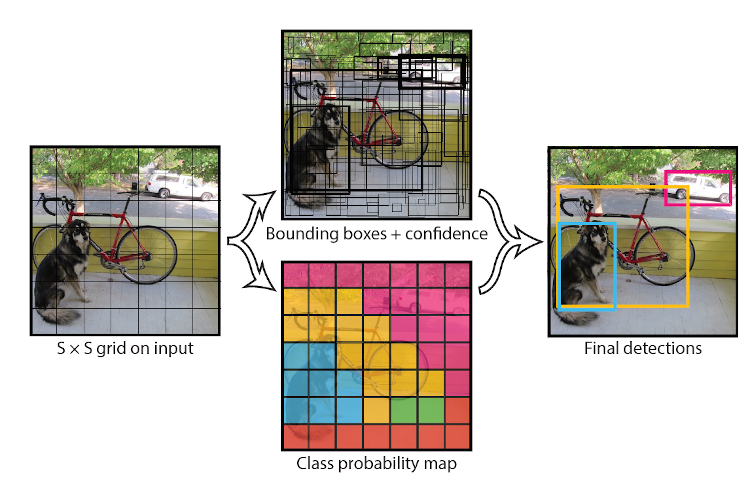
\includegraphics[width=15cm]{Bilder/yolo_model.png} 
		\caption[Vereinfachte Darstellung der Objekterkennung mit dem YOLO Algorithmus]{Vereinfachte Darstellung der Objekterkennung mit dem YOLO Algorithmus \cite{JosephRedmon.2016}}
		\label{yolo_model}
	\end{center}
\end{figure}

\subsubsection{YOLOv2}

\subsubsection{YOLOv3}




